\section{Durchführung}
\label{sec:Durchführung}
Die Stangen werden zunächst vermessen und gewogen.
Der Radius $r$ der runden Stange wird 10 mal mithilfe einer Schieblehre gemessen und später der Mittelwert gebildet.
Bei der Messung des Stabes mit recheckigem Querschnitt sind jeweils für Seite $a$ und $b$ 10 Messungen notwendig.
Zur Masse gehören zum einen die Gewichte, die Stange mit Gewinde und die Halterung an denen die Gewichte befestigt sind.

\subsection{Einseitige Einspannung}
\label{sec:einseitig}
Der Stab wird in der Apperatur wie in Abb. \ref{fig:apperatur} eingespannt.
Die Stäbe wurden schon häufiger gebogen und sind in der Ruheposition nicht mehr exakt gerade.
Daher wird zuerst die Durchbiegung des Stabes ohne Last $D_0(x)$ mithilfe der Messuhren vermessen.\\
Im Anschluss wird ein Gewicht $F$ am Ende des Stabes befestigt, so dass eine Auslenkung von $\SI{3}{\mm} - \SI{7}{\mm}$ erreicht wird.
Nun wird die Durchbiegung mit Masse $D_\text{M}(x)$ gemessen.
Die reale Durchbiegung beträgt dann
\begin{equation}
    D(x) = D_\text{M}(x) - D_0(x) .
    \label{eqn:D_real}
\end{equation}
Die Durchbiegung $D_0$ und $D_\text{M}$ soll für $15$ Abstände gemessen werden.
Dieser Vorgang wird für zwei Stäbe aus unterschiedlichem Material durchgeführt.
\begin{figure}
    \centering
    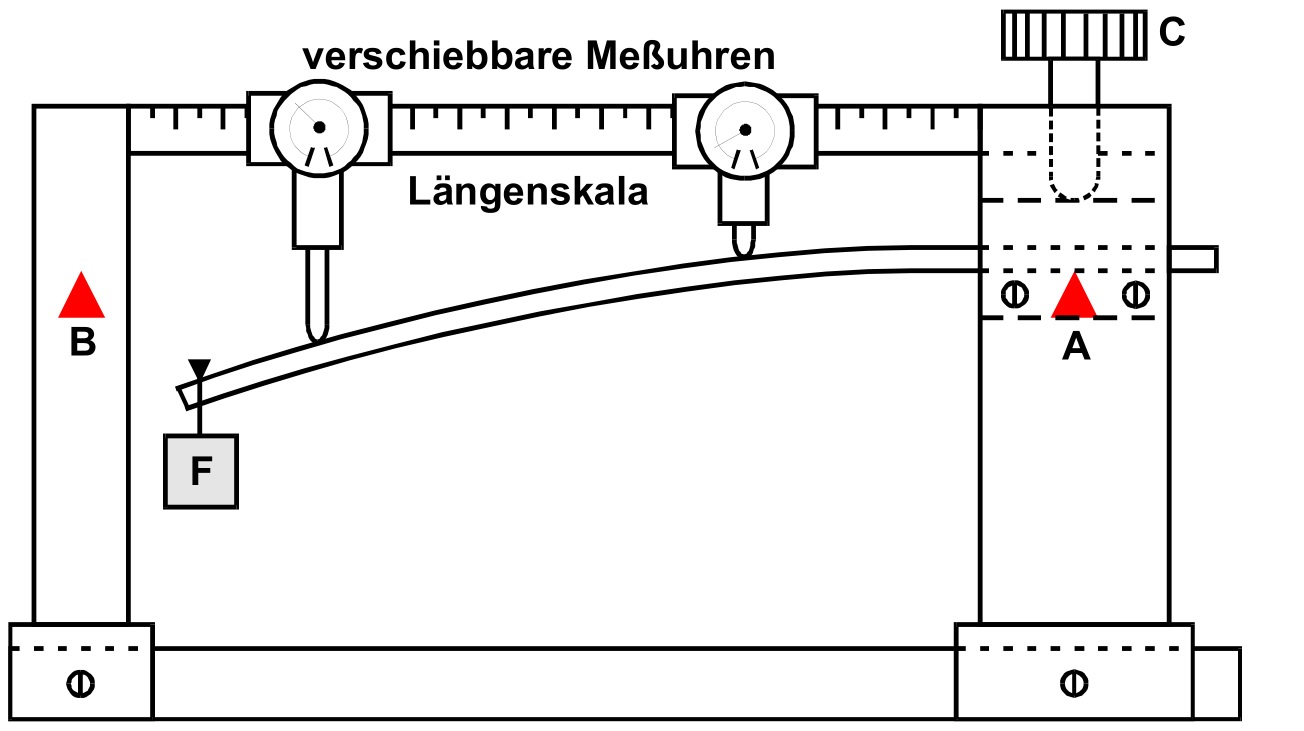
\includegraphics[width=0.75\textwidth]{content/data/apperatur.jpg}
    \caption{Darstellung der Apperatur zur einseitigen Biegung eines Stabes. \cite{anleitung}}
    \label{fig:apperatur}
\end{figure}

\subsection{Zweiseitige Biegung}
Der Stab wird diesmal in die Apperatur \ref{fig:apperatur} auf beiden Seiten (Punkt A und B) aufgelegt.
Zu beachten ist, dass die Stäbe diesmal nicht eingespannt werden dürfen.
Nun wird wie in \autoref{sec:einseitig} die Durchbiegung $D_0$ ohne Last gemessen.\\
Danach wird die Masse $m$ welche eine Kraft $F$ ausübt, in der Mitte der Auflagepunkte befestigt.
Hier wird mit einer Messuhr links und einer rechts von der Masse gemessen.
Die reale Durchbiegung ergibt sich aus der Differenz der Durchbiegung \eqref{eqn:D_real}.